\documentclass[titlepage]{scrartcl}
% Code Darstellung
\usepackage{listings}
\usepackage{listingsutf8}
\usepackage{multicol}

%lange Tabellen
\usepackage{longtable}
%Referenzen zwischen unterschiedlichen Dateien
\usepackage{xr}
%\externaldocument{theorie}
\usepackage{lscape}
%Deutsche Sprachunterstützung
\usepackage[utf8]{inputenc}
\usepackage[ngerman]{babel}
\usepackage{marvosym}
\DeclareUnicodeCharacter{20AC}{\EUR}

%Für das Einbinden von Bildern
\usepackage{graphicx}

%Tabellen
\usepackage{array}

%Tabellen automatisch schoener
\usepackage{booktabs}

%Caption
\usepackage{caption}
\usepackage{subcaption}

%Formeln
\usepackage{mathtools}
\usepackage{amsmath}
\usepackage{amssymb}
\usepackage{amstext}
\usepackage{dsfont}

%\usepackage{mnsymbol}

% Interssante natbib Optionen: 
% numbers : Nummerierte Zitateinheiten
% sort&compress : Bei mehrfachen Zitaten, Sortierung und ggf. Verkürzungen
%\usepackage[]{natbib}

%Vectorpfeile schöner
\usepackage{esvect}

%Formatierung
\usepackage[T1]{fontenc}
\usepackage{lmodern}
\usepackage{microtype}

%Schaltbilder malen
%\usepackage[europeanresistors,cuteinductors,siunitx]{circuitikz}
\usepackage{comment}
\usepackage{csquotes}

%Formatierungsanweisungen
\newcommand{\wichtig}[1]{\underline{\large{#1}}}
\newcommand{\aref}[1]{Abb. \ref{#1}}
\newcommand{\R}{\mathbb{R}}
\newcommand{\K}{\mathbb{K}}
\newcommand{\C}{\mathbb{C}}
\newcommand{\mr}[1]{\mathrm{#1}}

%Klickbare Referenzen
%\usepackage[hidelinks]{hyperref}
%\includeonly{theorie}
%\includeonly{theorie,versuchsdurchfuehrung,ergebnisse,anhang}
\begin{document}

\title{Eigenschaften optischer CCDs}
\subtitle{Gruppe 1}
\date{März 2014}
\author{Udo Beier \and Leon Brückner \and Valentin Olpp \and Sebastian Ziegler}

\maketitle
\tableofcontents
\newpage
\listoffigures
\listoftables
\newpage
%\section{Abstract}
\newpage
\section{Einleitung}
Bereits in der Schule lernt man, dass Licht aus verschiedenen Farben zusammengesetzt ist. Dies zeigt sich z.B. bei Prismen oder am natürlichen Phänomen des Regenbogens. 1814 hat Joseph von Fraunhofer im Sonnenspektrum schwarze Linien entdeckt.\footnote{\ \cite{ktroskopie}} Er konnte den Ursprung der nach ihm benannten Linien jedoch nicht erklären. Heutzutage ist der Ursprung der Linien bekannt. Die Linien entstehen dadurch, dass die Atome der Sonne nur das Licht bestimmter Frequenzen absorbieren können, was es erlaubt, aus Absorptions- oder Emissionsspektren von Licht auf Eigenschaften der Lichtquelle zu schließen. Das Zerlegen und Analysieren von Spektren wird als Spektroskopie bezeichnet und erlaubt die Erforschung vieler Eigenschaften von Himmelskörpern, wie z.B. die Bestimmung von Radialgeschwindigkeiten oder die Spektralklassifikation von Sternen. Im Folgenden wird sich deshalb mit der Spektroskopie beschäftigt.

%Quelle:   http://de.wikipedia.org/wiki/Spektroskopie

Für den elektromagnetischen Feldstärketensor gilt:
\begin{equation}
F^{\mu \nu} = \partial^{\mu} A^{\nu} - \partial^{\nu} A^{\mu}
\end{equation}
Dabei ist A das 4er-Verktorpotential.
Dies wird als Grundwissen vorausgesetzt und hier deshalb nicht weiter vertieft.
\section{Methoden}
\subsection{Zeitmaße}

Es existieren verschiedene Zeitmaße mit unterschiedlichen Definitionen, die im folgenden aufgeführt sind.
\begin{itemize}
\item Wahre Sonnenzeit (WZ): Die wahre Sonnenzeit wird am Stand der Sonne am Himmel gemessen und beträgt 12 Uhr, wenn die Sonne durch den Meridian des Standortes geht.
\item Mittlere Sonnenzeit (MZ): Die mittlere Sonnenzeit ist eine kurzfristig gleichmäßig vergehende Zeit, wobei eine fiktive mittlere Sonne den Zeitverlauf bestimmt. Sie läuft längs des Äquators
\item Weltzeit, Universal Time (UT): Die Weltzeit ist ein Zeitmaß, das aufgrund internationaler Vereinbarungen für jeden Ort die gleiche Zeit liefert. Sie entspricht dabei der mittleren Sonnenzeit auf dem 0-Meridian.
\item Zonenzeit: Als Zonenzeit wird eine einheitliche Zeit innerhalb einer Zeitzone bezeichnet. Dabei wird die Erde in 24 Zeitzonen eingeteilt, um innerhalb einer Zeitzone vertretbare Abweichungen von der mittleren Sonnenzeit zu gewährleisten.
\item Julianisches Datum (JD): Das Julianische Datum gibt die Tage an, die seit dem 1. Januar -4712, 12 Uhr vergangen sind.
\item Sternzeit, Sidereal Time (ST): Die Sternzeit ist ein Zeitmaß, das auf der scheinbaren Rotation der Sterne am Himmel, hervorgerufen durch die Erdrotation, beruht. Ein Sterntag ist die Dauer, die der Sternenhimmel für ein ganze scheinbare Umdrehung benötigt. Die ST definiert sich als Stundenwinkel des Frühlingspunkts.
\item Ephemeridenzeit (ET,TT oder TDT): Die Ephemeridenzeit ist ein durch die Dynamik des Sonnensystems definiertes Zeitmaß. Eine Ephemeridensekunde entspricht dabei dem 31.556.925,9747ten Teil des Tropischen Jahres 1900. 
\item Atomzeit: Die Atomzeit ist ein Zeitmaß das auf der SI-Sekunde basiert und wird weltweit bei zahlreichen Zeitinstituten in der Regel durch Cäsium-Atomuhren realisiert. Eine Sekunde ist das 9.192.631.770-fache der Periodendauer der dem Übergang zwischen den beiden Hyperfeinstrukturniveaus des Grundzustandes von Atomen des Nuklids Cs-133 entsprechenden Strahlung.
\end{itemize}

Dabei verlaufen die Ephemeridenzeit und die Atomzeit streng gleichförmig, ungleichmäßig dagegen verlaufen die mittlere Sonnenzeit, die Weltzeit und die Zonenzeit aufgrund der Schwankungen der Erdrotation.

Die wahre Sonnenzeit verläuft aus zwei Gründen ungleichmäßig: Zum einen wird der gleichmäßige Verlauf durch die elliptische Form der Erdbahn und zum anderen durch die Neigung der Erdachse gestört.

Die Sternzeit steht unter dem Einfluss von Schwankungen der Rotation der Erde, wie z.B. die Präzession. Daher verläuft die Sternzeit nicht streng gleichförmig.

\subsection{Astronomische Koordinatensysteme}
Für diese Messung sind drei Koordinatensysteme von besonderer Bedeutung.

\subsubsection{Horizontsystem}

Der Ursprung des Horizontsystems liegt beim Beobachter, der Grundkreis ist der lokale Horizont. Längen- und Breitenkoordinaten entsprechen Höhenwinkel und Azimut. Die Pole sind Zenit und Nadir, wesentlicher Verwendungszweck sind Messungen an der Erdoberfläche. 

\subsubsection{Festes Äquatorsystem}

Beim festen Äquatorialsystem liegt der Ursprung wahlweise im Beobachter oder im Erdmittelpunkt. Der Grundgkreis ist hier der Himmeläquator, Längen- und Breitengrad entsprechen Deklinations- und Stundenwinkel. Die Pole sind die Himmelspole selbst. Verwendet wird dieses System vor allem bei astronomischen Beobachtungen. 

\subsubsection{Bewegliches Äquatorsystem}

Das bewegliche Äquatorialsystem entspricht dem festen, bis auf den Unterschied, dass Längen- und Breitengrad Deklinationswinkel und Rektazension entspricht. 

\subsection{Azimut und Deklination}
In einem Koordinatensystem mit einer Grundebene, welche im Fall etwa des Horizontsystems die Erdoberfläche ist, und einem dazu senkrechten Zenit, definiert man die Deklination als den Winkel zwischen Objekt und der Grundebene, sowie den Azimut als Winkel relativ zu einer ausgezeichneten Richtung. Im Fall des Horizontsystems ist dies etwa die Nord-Süd-Richtung, wobei 0 $^\circ$ Süden entspricht und die Zählung über Westen, Norden und Osten fortgesetzt wird.  

\subsection{Der Theodolit}
Für die Bestimmung der relativen Azimutwerte wird ein Theodolit verwendet, welcher mittels einer Montierung auf den Teleskopsäulen im Garten befestigt werden kann. An der Montierung wird ein Element in Form eines regelmäßigen Dreiecks befestigt, das mittels zweier Feinhorizontierschrauben relativ zur Montierung bewegt werden kann, allerdings nur um sehr kleine Wege. Dieser Mechanismus dient der Feineinstellung. Der Rest des Theodoliten ist mit einem Kugelgelenk mit dem vorherigen Element verbunden. \\
Daran schließt sich der eigentliche Theodolit an: Dieser ist zum einen drehbar um die vertikale Achse, zum anderen drehbar um eine horizontale Achse gelagert, sodass nun jeder beliebige Punkt am Himmel durch das sich anschließende Fernrohr anvisiert werden kann.  Des weiteren existiert eine Einrichtung zur Einstellung des Nullpunktes der Azimut-Skala sowie eine Wasserwaage, mit der die horizontale Ausrichtung des Theodoliten geschieht. \\
Im ersten Schritt soll der Theodolit horizontal ausgerichtet werden, sodass sich also bei einer Drehung des Theodoliten um die vertikale Achse nur der Azimut des betrachteten Objekts ändert und nicht dessen Deklination.\\
Dazu wird zunächst der Theodolit mittels des Kugelgelenks und einer Libelle (kreisförmige \enquote{Wasserwaage}) grob horizontal ausgerichtet. Die Feinjustierung geschieht dann mittels eines Algorithmus, mit dem man sich der horizontalen Ausrichtung annähert: Zunächst wird die Wasserwaage entlang einer Seite der dreieckigen Grundfläche ausgerichtet und die Ausrichtung des Theodoliten mit der entsprechenden Feinhorizontierschraube exakt auf Null eingestellt. Danach wird der Theodolit um 180 $^\circ$ um die vertikale Achse gedreht und der neue Ausschlag der Luftblase mittels der gleichen Feinjustierschraube halbiert. Anschließend wird der Theodolit um selbige Achse nochmals um 90 $^\circ$ gedreht und der Ausschlag der Luftblase mit der zweiten Feinhorizontierschraube auf den vorherigen Spielpunkt eingestellt. Indem dieses Vorgehen wiederholt wird, erreicht man nach ausreichend vielen Wiederholungen eine hinreichend genaue horizontale Justierung des Theodoliten. \\

\subsection{Messungen mit dem Theodoliten}
Azimut und Deklination eines Objekts können bestimmt werden, indem das entsprechende Objekt anvisiert wird. Durch Umlegen eines Schalters kann man zwischen Deklination und Azimut wechseln. Der entsprechende Wert kann dann durch das Mikroskoprändel angelesen werden. Dazu muss die Mikrometertrommel derart eingestellt werden, dass die Lücken in den beiden sichtbaren Balken exakt nebeneinander liegen. 

\subsection{Messung des Turmazimuts}
Mit einem derart justierten Theodoliten können nun Azimut und Deklination eines Objekts am Himmel bestimmt werden, indem man das entsprechende Objekt anvisiert und auf der Skala nun den jeweiligen Winkel, der in gon angezeigt wird, abliest. Dabei kann die Deklination als absoluter Wert im Horizontsystem abgelesen werden, wohingegen der Azimut nur relativ zu einem frei einstellbaren Nullpunkt bestimmbar ist. \\
Um nun den Azimut des angesprochenen Objekts zu bestimmen, wird nun der relative Azimut des Objekts sowie der Azimut eines anderen Objekts abgelesen, der beispielsweise mittels Literatur- und Tabellenwerten als absoluter Wert bestimmt werden kann. Dieses zweite Objekt ist in diesem Fall die Sonne. \\
Um den Turmazimut zu bestimmen, wird das Objekt mittels des Fadenkreuzes derart anvisiert, dass sich die Turmspitze möglichst exakt zentral im Fadenkreuz befindet. \\

\subsection{Messung des Sonnenazimuts}
Da die Sonne nicht direkt durch das Fernrohr beobachtet werden kann, da dies zu einer sofortigen Schädigung des Auges und der Sehfähigkeit führen würde, muss hierfür ein Filter verwendet werden. Bei der Messung wurden eine Kombination aus einem UV-IR-Rejection-Filter sowie aus zwei Neutraldichte-Filtern mit den Werten 1.8 und 3.0 eingesetzt. \\ 
Zur Bestimmung des Sonnenazimuts wird ein Überstreichen der Sonnenscheibe über einen senkrechten Strich des Fadenkreuzes betrachtet. Mit einer Stoppuhr wird eine Zeitmessung gestartet, wenn der rechte Rand der Sonnenscheibe jenen Strich berührt. Wenn der linke Rand den gleichen Strich überstreicht, wird eine Zwischenzeit genommen, zu einem frei gewählten Zeitpunkt, der ebenfalls notiert wird, wird schließlich die Messung beendet. Aus diesen drei Messungen kann der Zeitpunkt in MEZ bestimmt werden, an dem das Zentrum der Sonnenscheibe das Zentrum des Fadenkreuzes überstreicht. Der Zeitpunkt, zu dem das Zentrum der Sonne das Zentrum des Fadenkreuz überstreicht, kann einfach mittels der folgenden Formel bestimmt werden: 
\begin{equation}
U_{zen} = U_{end} - (t_{end} - \frac {t_{zw}}{2}), 
\end{equation}
wobei $U_{zen}$ die Uhrzeit des Zentrumdurchgangs, $U_{end}$ die Uhrzeit bei Beendigung der Messung, $t_{end}$ die von der Stoppuhr am Ende der Messung angezeigte Zeit sowie $t_{zw}$ die gemessene Zwischenzeit auf der Stoppuhr. 

\subsection{Berechnung des absoluten Sonnenazimuts}
Mittels der in ... dargestellen Berechnung kann aus Tabellenwerten für die Sternzeit um 0 Uhr des Messtages in Greenwich, den aktuellen Offset zwischen universal time (UT) und Ephemeridenzeit (TT) sowie den Werten für die Sonnendeklination und den Sonnenazimut im Äquatorialsystem zu Beginn und Ende des Messtages der absolute Azimut der Sonne zu jedem Messzeitpunkt eines Wertes für den Sonnenazimut bestimmt werden. Daraus ergibt sich durch Mittelung der Offset zwischen dem eingestellten Nullpunkt des Azimuts und der Nord-Süd-Verbindung. 
Durch Addition des Unterschiedes zwischen den relativen Azimutwerten für Turm und Sonne kann so der absolute Azimut des Turms bestimmt werden. 
\section{Ergebnisse}
\subsection{Npoint-Scan der Sonne}
Der npoint Scan ergab, dass das Intensitätsmaximum der Sonne einen Offset zur in der Katalogdatei für die Sonne eingetragenen Position aufwies. Abbildung %\ref{npoint_sun} zeigt einen Plot des npoint Scans.
Die Auswertung des Cross-Scans zeigte, dass das Maximum des Elevationsscans um 3241,6 niedriger ausfiel als das Maximum des Azimutscans. Die Position des Maximums war an der durch den npoint Scan ermittelten Stelle.

\subsection{Cross-Scan der Sonne}
bla bla (wie daten entstanden, wie fehlerbalken entstanden)

\begin{figure}
		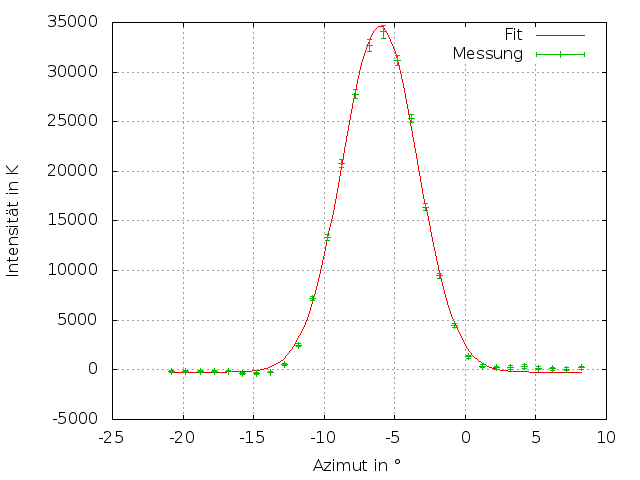
\includegraphics[width=.9\textwidth]{images/sun_azimut}
\caption{ Plot der Intensität der Sonne in Abhängigkeit des Azimutwinkels }
\label{fig:sunaz}
\end{figure}

\begin{figure}
		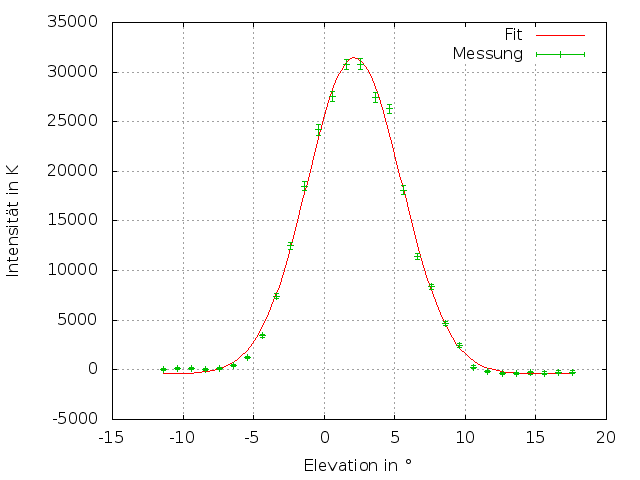
\includegraphics[width=.9\textwidth]{images/sun_elevation}
\caption{ Plot der Intensität der Sonne in Abhängigkeit des Elevationswinkels }
\label{fig:sunel}
\end{figure}

\subsection{Bestimmung der Halbwertsbreite der Antennenkeule}
Zur Bestimmung der Halbwertsbreite der Antennenkeule wurden die Messdaten mit einer Gauß-Funktion gefittet (siehe Abb. \ref{fig:sunaz} und \ref{fig:sunel}). Für die Funktion

\begin{equation}
f(x) = a \cdot e^{- \frac{(x-d)^2}{b}} + c
\label{form:FWHMfit}
\end{equation}

ergaben sich dabei Werte, wie in Tabelle \ref{tab:FWHM} zu sehen.

\begin{table}
\centering
\begin{tabular}{ccc}
Parameter	&			Wert der Azimutmessung	&	Wert der Elevationsmessung \\
\midrule
a			&			34861 $\pm$ 274			&	31855 $\pm$ 393 \\
b			&			14.32 $\pm$ 0.29		&	22.29 $\pm$ 0.72 \\
c			&			-226.4 $\pm$ 117.0		&	-401.9 $\pm$ 207.3 \\
d			&			-6.045 $\pm$ 0.023		&	2.146 $\pm$ 0.045
\end{tabular}
\caption{Werte des Fits für die Parameter aus \eqref{form:FWHMfit}}
\label{tab:FWHM}
\end{table}

Bei dieser Gauß-Funktion ergibt sich die Halbwertsbreite H folgendermaßen:

\begin{equation}
H = 2 \sqrt{2 \ln 2} \cdot \sqrt{\frac{b}{2}}
\end{equation}

Durch Fehlerfortpflanzung ergibt sich:

\begin{equation}
\delta H = \frac{\sqrt{2 \ln 2}t}{2} \sqrt{\frac{2}{b}} \cdot \delta b
\label{form:FehlerFWHM}
\end{equation}

Aus \eqref{form:FehlerFWHM} ergibt sich dann:

\begin{align*}
H_{\mr{Azimut}} = 6.300\,^\circ \ &\mathrm{und} \ \delta H_{\mr{Azimut}} = 0.062\,^\circ \\
H_{\mr{Elevation}} = 6.545\,^\circ \ &\mathrm{und} \ \delta H_{\mr{Elevation}} = 0.106\,^\circ
\end{align*}

Zusammenfassend ergibt sich also:

\begin{align}
H_{\mr{Azimut}} = 6.30\,^\circ \pm 0.07\,^\circ \\
H_{\mr{Elevation}} = 6.54\,^\circ \pm 0.11\,^\circ
\end{align}

Aufgrund der Rotationssymmetrie der Antennenkeulen, lässt sich die Halbwertsbreite der Keulen durch Mittelwertbildung bestimmen. Dabei folgt aus $ H = \left(H_{\mr{Azimut}} + H_{\mr{Elevation}}\right)/2 $ mittels Fehlerfortpflanzung:

\begin{equation}
\delta H = \frac{\sqrt{{\delta H_{\mr{Azimut}}}^2 + {\delta H_{\mr{Elevation}}}^2}}{2}
\end{equation}

Daraus erhält man:

\begin{equation}
H = 6.4226\,^\circ \pm 0.0616\,^\circ \approx 6.42\,^\circ \pm 0.07\,^\circ
\end{equation}
%\section{Diskussion}
Für die ideale Betriebstemperatur des CCD-Chips ergab sich hier ein Wert von -15 $^\circ$ C, der allerdings durch die eingeschränkte Kühlleistung der Kamera nach unten beschränkt ist. Würde man eine verbesserte Kühlung verwendet, so wäre eine tiefere Temperatur und wahrscheinlich auch ein noch geringerer Dunkelstrom zu erwarten. \\
Der geplottete Verlauf entspricht weitgehend den theoretischen Erwartungen: \\
Die Elektronen im Halbleitermaterial sind boltzmann-verteilt, die Anzahl pro Energie und Temperatur geht also mit $exp(-\frac{E}{k \cdot T})$. Der exponentielle Anstieg des Dunkelstroms mit der Temperatur findet sich auch im entsprechenden Plot wieder. \\
Der offset der Exponentialfunktion ist wahrscheinlich auf den bias des CCD-Chips zurückzuführen, also den ADU-Wert, der auch bei minimaler Belichtungszeit und geschlossener Blende messbar ist. \\
Bei der Berechnung des Gain-Faktors ergibt sich zwar eine Tendenz bei unterschiedlichen Belichtungszeiten, allerdings ist der Fehler des Gain-Faktors verhältnismässig klein. Für eine Verbesserung der Bestimmung des Gain-Faktors dürfte eine genauere Aufschlüsselung der Beiträge zur Streuung hilfreich sein, sodass eine genauere Bestimmung von $\sigma^{stat}$ möglich sein dürfte. \\
Bei der Betrachtung des ADU-Outputs über der Intensität des eingestrahlten Lichts ergibt sich in guter Näherung eine lineare Abhängigkeit. Allerdings sind die ADU-Werte für grössere Intensitäten geringer als durch Interpolation des linearen Verlaufs zu erwarten wäre. Grund hierfür kann sein, dass bei großen Intensitäten einige Pixel der Aufnahme doch überbelichtet sind, sodass hier der ADU-Wert konstant bei dem Maximalwert von etwa 65500 liegt. Des weiteren wurde bei der Auswertung ein Rechteck, das genau die Diode einschloss, betrachtet und aufintegriert. Hierbei ist zunächst der von der von der eingestrahlten Intensität unabhängige Dunkelstrom ein Fehler, der insbesondere bei geringen Helligkeiten eine zunehmend große Rolle spielt. Weiter ist es bei den kaum belichteten Aufnahmen schwierig, die Diode exakt \enquote{einzurahmen}, sodass hier unterschiedliche Bereiche betrachtet werden. Dieser Fehler könnte vermieden werden, indem man leichte Störungen der Anordnung von Diode und Kamera verhindert und anschließend immer den gleichen Bildausschnitt betrachtet. Eine weitere Fehlerquelle können auch die Filter sein, die möglicherweise nicht exakt den angegebenen Absorptionsgrad aufweisen. \\
Eventuell könnte die Messung verbessert werden, indem man statt einer Diode mit großem Helligkeitsgradienten eine homogen ausgeleuchtete Fläche verwendet, da hier überbelichtete Pixel verhindert werden können. Des weiteren wäre es sinnvoll, von den Diodenaufnahmen einen passenden dark frame zu subtrahieren, sodass der Dunkelstrom keinen Fehler mehr liefert. \\
Tatsächlich liefert der Versuch aber das erwartete Ergebnis. 
%\section{Aufgabe 5}
Die Erde dreht sich in 23 Stunden, 56 Minuten und 4.1 Sekunden einmal um ihre eigene Achse bzw. die Stundenwinkelachse.
Die Winkelgeschwindigkeit der Erde ergibt sich dann zu:
\begin{equation}
\omega_{Erde} = \frac{2\pi}{T} = \frac{2\pi}{86164.1 \mathrm{s}} \approx 7.30 \cdot 10^{-5} \frac{1}{\mathrm{s}}
\end{equation}
bzw. $4.18 \cdot 10^{-3\   \circ} \frac{1}{\mathrm{s}}$.
Der Mond dreht sich in 27.56 Tagen (anomalistische Periode) einmal um die Erde. Seine Winkelgeschwindigkeit $\omega_{Mond}$ aus Sicht der Erde ergibt sich damit zu $2.64\cdot 10^{-6} \frac{1}{\mathrm{s}}\ \textrm{bzw.}\ 1.51 \cdot 10^{-4\   \circ} \frac{1}{\mathrm{s}}$.
Die Winkelgeschwindigkeit, mit der der Mond durch das Sichtfeld des Teleskops (bei ausgeschalteter Nachführung) wandert, ergibt sich damit zu $\omega = \omega_{Erde}-\omega_{Mond}$, also zu $7.04\cdot 10^{-5} \frac{1}{\mathrm{s}}$ bzw. $4.03 \cdot 10^{-3\   \circ} \frac{1}{\mathrm{s}}$. 
Der Winkeldurchmesser des Mondes ergibt sich über die Beziehung
\begin{equation}
tan\  \alpha_{Mond} = \frac{D_{Mond}}{d_{Erde-Mond}}
\end{equation}
wobei $D_{Mond}$ der Durchmesser des Mondes und $d_{Erde-Mond}$ die mittlere Entfernung von Erde und Mond ist, von der der Radius der Erde abgezogen wurde.
Mit Kleinwinkelnäherung gilt dann:
\begin{equation}
\alpha_{Mond} = \frac{D_{Mond}}{d_{Erde-Mond}} = \frac{3476 \mathrm{km}}{387129 \mathrm{km}} \approx 8.98 \cdot 10^{-3}\ \mathrm{bzw.}\ 0.51^{\circ} = 30' 22''
\end{equation}
\\
Die Zeit, die der Mond braucht, um das Sichtfeld des Teleskops zu durchwandern, hängt vom verwendeten Teleskop und Okular ab.
Als allgemeine Formel gilt:
\begin{equation}
t = \frac{\alpha_{Teleskop}+\alpha_{Mond}}{\omega}
\end{equation}
$\alpha_{Teleskop}$ ergibt sich aus der Formel
\begin{equation}
\alpha_{Teleskop} = \frac{\alpha_{Schein}}{V}
\end{equation}
wobei $\alpha_{Schein}$ das scheinbare Sichtfeld des Okulars und V die erreichbare Vergrößerung des Teleskops ist. V errechnet sich aus
\begin{equation}
V = \frac{f_{Teleskop}}{f_{Okular}}
\end{equation}
wobei f die Brennweite des Teleskops bzw. des Okulars ist.
\\
Also gilt:
\begin{equation}
t = \frac{\frac{f_{Okular}}{f_{Teleskop}}\cdot \alpha_{Schein} + \alpha_{Mond}}{\omega}
\end{equation}

Als Beispiel soll nun die Zeit für das 50cm - Teleskop ($f_{Teleskop} = 3.35\mathrm{m}$) mit dem Universal-Zoomokular einmal bei minimalem ($\alpha_{Schein}=48^{\circ}, f_{Okular} = 24 \mathrm{mm}$) und maximalem ($\alpha_{Schein}=68^{\circ}, f_{Okular} = 8 \mathrm{mm}$) Zoom berechnet werden.
\begin{equation}
t_{minZoom} = \frac{\frac{24 \cdot 10^{-3} \mathrm{m}}{3.35 \mathrm{m}}\cdot \frac{4}{15}\pi + 8.98 \cdot 10^{-3}}{7.04\cdot 10^{-5} \frac{1}{\mathrm{s}}} \approx 213 \mathrm{s}
\end{equation}
\begin{equation}
t_{maxZoom} = \frac{\frac{8 \cdot 10^{-3} \mathrm{m}}{3.35 \mathrm{m}}\cdot \frac{17}{45}\pi + 8.98 \cdot 10^{-3}}{7.04\cdot 10^{-5} \frac{1}{\mathrm{s}}} \approx 168 \mathrm{s}
\end{equation}

\section{Aufgabe 6}
Damit die beiden Sterne eines visuellen Doppelsterns noch unterschieden werden können, muss das \textbf{Rayleigh-Kriterium} gelten:
\begin{equation}
\beta \approx 1.22\frac{\lambda}{d}
\end{equation}
Hier ist $\beta$ der von der Erde aus gesehene Winkel zwischen den beiden Sternen, $\lambda$ die Wellenlänge des Lichts und $d$ der Durchmesser des Teleskops. Wenn zwei Sterne unter einem kleineren Winkel erscheinen, können sie nicht mehr auseinander gehalten werden.
Es gibt auch noch das empirisch gefundene \textbf{Dawes-Kriterium}:
\begin{equation}
\beta \approx \frac{12''}{d}
\end{equation}
wobei $d$ der Durchmesser des Teleskops in cm ist.
\\
Das Sichtfeld berechnet sich aus:
\begin{equation}
\alpha = \frac{f_{Okular}}{f_{Teleskop}}\cdot \alpha_{Schein}
\end{equation}
\begin{enumerate}
\item
50 cm - Teleskop
$\alpha_{min} = 0.16^{\circ}$
$\alpha_{max} = 0.34^{\circ}$
\item
40 cm - Teleskop
$\alpha_{min} = 0.14^{\circ}$
$\alpha_{max} = 0.29^{\circ}$
\item
APO - Refraktor
$\alpha_{min} = 0.68^{\circ}$
$\alpha_{max} = 1.43^{\circ}$
\end{enumerate}




Es gilt für die scheinbare Helligkeit und bei konstantem Abstand: 
\begin{equation}
m_2 - m_1 = 2.5\cdot \log(\frac{L_1}{L_2}). 
\end{equation}, 
wobei $m_1, m_2$ die scheinbaren Helligkeiten und $L_1, L_2$  die Leuchtkräfte der beiden Sterne im gleichem Abstand zum Beobachter sind.

Durch Umformung ergibt sich: 
\begin{equation}
\frac{L_1}{L_2} = 10^{\frac{(m_2 - m_1)}{2.5}}. 
\end{equation}

Für ein Doppelstern mit den scheinbaren Helligkeiten $m_1$ und $m_2$ ergibt sich also: 
Die Gesamtleuchtkraft ergibt sich durch Addition der einzelnen Leuchtkräfte und die Gesamtmagnitude nach Umrechnung der Gesamthelligkeit. 

\begin{equation}
L_{ges} = L_1 + L_2 = L_1 \cdot (1 + \frac{L_2}{L_1}) = L_1 \cdot (1 + 10^{\frac{(m_1 - m_2)}{2.5}}). 
\end{equation}

Für die Gesamtmagnitude ergibt sich:
\begin{equation}
m_{ges} = m_1 - 2.5\cdot \log(\frac{L_{ges}}{L_1}) = m_1 - 2.5\cdot \log(1 + 10^{\frac{(m_1 - m_2)}{2.5}}).
\end{equation}. 
Die beiden Doppelsterne, die in den vorhergehenden Aufgaben vorkommen, sind $\gamma$ And und $\gamma$ Leo, bei denen die beiden Hauptsterne eine scheinbare Helligkeit 
\bibliographystyle{natdin}
%\begin{thebibliography}{9}
%\bibitem[Bec]{kmann} BECKMANN, Dieter. Astrophysik. C.C.Buchner, 2011.
\bibitem[Spe]{ktroskopie} Wikipedia: Spektroskopie. Online im Internet: URL: http://de.wikipedia.org/wiki/Spektroskopie (Stand: 11.03.2014). 
\bibitem[Ast]{ronomischesPraktikum} Astronomisches Praktikum.
\end{thebibliography}

\newpage
%\bibliographystyle{natdin}
%\bibliography{literature}
%\section{Anhang}

\begin{table}[h!]
\centering
\begin{tabular}{c|c|c|c}
Winkel Sonne & Zwischenzeit (h min s) & Endzeit (h min s) & MEZ Funkuhr \\ 
\hline 
180 $^\circ$  13' 54'' & $2^m 16.18^s$  & $2^m 59.18^s$ & $10^h 52^m 00^s$ \\ 

182 $^\circ$  29' 01'' & $2^m 14.44^s$  & $3^m 00.03^s$ & $10^h 59^m 30^s$ \\ 

183 $^\circ$  37' 44'' & $2^m 14.18^s$  & $2^m 44.53^s$ & $11^h 03^m 00^s$ \\ 

184 $^\circ$  50' 08'' & $2^m 13.75^s$  & $2^m 48.85^s$ & $11^h 07^m 00^s$ \\ 

189 $^\circ$  03' 04'' & $2^m 12.44^s$  & $2^m 48.78^s$ & $11^h 20^m 30^s$ \\ 

190 $^\circ$  13' 49'' & $2^m 11.83^s$  & $3^m 05.00^s$ & $11^h 24^m 30^s$ \\ 

191 $^\circ$  45' 55'' & $2^m 11.68^s$  & $3^m 16.66^s$ & $11^h 29^m 30^s$ \\ 

193 $^\circ$  07' 52'' & $2^m 11.00^s$  & $2^m 31.37^s$ & $11^h 33^m 00^s$ \\

\end{tabular} 
\label{tab:sun}
\caption{Messung des Sonnenazimut}
\end{table}

\begin{table}[h!]
\centering
\begin{tabular}{c}

Gemessener Azimut \\
\hline
117 $^\circ$ 40' 24'' \\ 

117 $^\circ$ 40' 24'' \\ 

117 $^\circ$ 40' 22'' \\ 

117 $^\circ$ 40' 23'' \\ 

117 $^\circ$ 40' 24'' \\ 

117 $^\circ$ 40' 22'' \\ 

117 $^\circ$ 40' 24'' \\ 

117 $^\circ$ 40' 22'' \\ 

\end{tabular}
\caption{Messung des Turmazimut}
\label{mess_turm}
\end{table}


\begin{table}[h!]
\centering
\begin{tabular}{c}
Berechneter Sonnenazimut \\
\hline
330.207231345\\
332.460255182\\
333.606001818\\
334.812139975\\
339.025513227\\
340.206071994\\
341.739111616\\
343.104060402\\
\end{tabular}
\caption{Berechneter Sonnenazimut}
\label{sonnenaz}
\end{table}

\begin{thebibliography}{9}
\bibitem[Ast] {astr} Astronomisches Praktikum. Modul \enquote{Einführung in die Astronomie}. Dr. Karl Remeis Sternwarte. Bamberg
\bibitem[Jan] {sky} Jansky, K.G.\ 1933, nature, 132, 66 
\bibitem[Ray] {Ray} Wikipedia. Rayleigh-Jeans-Gesetz. https://de.wikipedia.org/wiki/Rayleigh-Jeans-Gesetz. (27.2.2014, 15 Uhr)
%\bibitem[Wik] {ipediaCCD} http://de.wikipedia.org/wiki/CCD-Sensor
%\bibitem[Ber] {ry} The Handbook of Astronomical Image Processing, Richard Berry, James Burnell, Willmann-Bell 2006.
\end{thebibliography}
\end{document}